\documentclass[11pt,a4paper]{article}
\usepackage[T1]{fontenc}
\usepackage[utf8]{inputenc}
\usepackage[brazil]{babel}
\usepackage{lmodern}
\usepackage[margin=2cm]{geometry}
\usepackage{microtype}
\usepackage{graphicx}
\usepackage{float}
\usepackage{booktabs}
\usepackage{array}
\usepackage{adjustbox}
\usepackage{amsmath}
\usepackage{amssymb}
\usepackage[font=small,labelfont=bf,skip=3pt]{caption}
\usepackage{fancyvrb}
\usepackage{upquote}
\usepackage{xcolor}
\usepackage{enumitem}
\usepackage[colorlinks=true,linkcolor=blue,urlcolor=blue,citecolor=blue]{hyperref}

\setlist{nosep,leftmargin=*,topsep=2pt}
\setlength{\parskip}{3pt}
\setlength{\parindent}{0pt}
\DefineVerbatimEnvironment{codigo}{Verbatim}{fontsize=\scriptsize,frame=single,rulecolor=\color{gray!60}}
\newcommand{\destaque}[1]{\begin{center}\fcolorbox{blue!50}{blue!5}{\parbox{0.96\linewidth}{#1}}\end{center}}
\emergencystretch=3em

\title{\vspace{-1.2cm}Detecção de Intrusão em Redes (NSL-KDD) --- Relatório Final}
\author{\small Gabriel Egídio Santos Beloni \quad Gabriel Evangelista Massara \quad Pedro Henrique Cardoso Maia \quad Pedro Tinoco Lanna\\[2pt]
\small Inteligência Artificial --- Profa. Cristiane Neri Nobre --- Trabalho em competição (grupo 7)\\[2pt]
\small \href{https://colab.research.google.com/drive/1cB8Rp90htsr9atA2CzmL1xEUhZNPjBiv?usp=sharing}{Notebook 04 no Google Colab} \quad$\cdot$\quad
\href{https://github.com/pedro-maia1337/IA-CopaLibertadores/blob/main/results/submissao_7.csv}{\texttt{submissao\_7.csv} no GitHub} \quad$\cdot$\quad
\href{https://github.com/pedro-maia1337/IA-CopaLibertadores}{Repositório}}
\date{\vspace{-1cm}}

\begin{document}
\shorthandoff{"}
\maketitle

\destaque{\textbf{F1-macro esperado no teste: 0,8819 $\pm$ 0,0030}, estimado por validação cruzada no treino (5 folds $\times$ 3 repetições), agrupada por linhas duplicadas e calculada em todas as linhas, como a métrica oficial. Modelo final: \emph{HistGradientBoosting} com categorias e ausentes nativos, limpeza de redundâncias no treino e limiar de decisão ajustado. Fora das linhas com rótulo contraditório, o modelo acerta 99,8\% das conexões.}

% =====================================================================
\section{Problema, base e diagnóstico}

O objetivo é classificar conexões de rede como \texttt{normal} ou \texttt{anomaly} a partir de 41 atributos de tráfego. A métrica oficial é o F1-macro, a média simples do F1 das duas classes. Usamos o F1-macro, e não a acurácia, porque a base é muito desbalanceada: só 5,8\% das 69.833 linhas de treino são ataques, e um modelo que dissesse ``normal'' para tudo teria 94,2\% de acurácia, mas F1-macro de apenas 0,485. A análise exploratória (Etapa 1) mostrou cinco problemas, que guiaram todo o trabalho:

\begin{itemize}
\item \textbf{Colunas de vazamento.} \texttt{score\_ids\_legado}, \texttt{tipo\_alerta\_soc} e \texttt{tempo\_resposta\_analista\_min} são registradas depois do evento (alerta do SOC e tempo de resposta do analista). Sozinhas, sem nenhum dado de rede, chegam a F1-macro de 0,889, acima dos 0,875 de um modelo com os 41 atributos de rede. São cópias ruidosas do rótulo e foram \textbf{excluídas}, assim como cinco colunas que são cópias exatas de outras (por exemplo, \texttt{src\_bytes\_kb}).
\item \textbf{Redundância e inconsistência.} 18,7\% das linhas são cópias, e há \textbf{1.702 grupos de linhas idênticas com rótulos opostos} (3.730 linhas).
\item \textbf{Ausentes.} 24 dos 41 atributos têm valores ausentes (40\% em \texttt{src\_bytes}), e 93,8\% das linhas têm ao menos um.
\item \textbf{Valores impossíveis} em 8,1\% das linhas: taxas acima de 1, contagens acima do limite da janela e valores negativos.
\item \textbf{Grafias variantes} nos categóricos (``TCP'', ``tcp''), padronizadas na leitura: \texttt{service} fica com 67 categorias.
\end{itemize}

% =====================================================================
\section{Metodologia e prevenção de vazamento}

\begin{itemize}
\item \textbf{Pipeline único.} Todo passo que aprende algo dos dados (remoção de redundâncias, imputação, codificação, escala, redução e balanceamento) é uma etapa de um \texttt{Pipeline} do \emph{imbalanced-learn}. Assim, na validação cruzada, cada passo é ajustado só com os folds de treino, e os passos que removem ou criam linhas nunca tocam a validação nem o teste.
\item \textbf{Validação cruzada agrupada.} Usamos \texttt{StratifiedGroupKFold} com 5 folds, estratificado pela classe e \textbf{agrupado por duplicata}: linhas idênticas ficam sempre no mesmo fold. Sem isso, o modelo seria avaliado em cópias de linhas que já viu, e a nota sairia inflada.
\item \textbf{Métrica em todas as linhas e limiar cruzado.} O F1-macro de cada fold é calculado em todas as linhas, com cópias e conflitos, como a professora faz no teste. O limiar de decisão de cada fold é escolhido nas previsões dos \emph{outros} folds.
\item \textbf{Regra de decisão declarada antes dos testes.} Em cada comparação, partimos da opção mais simples e só a trocamos por uma alternativa que a superasse em mais de um desvio-padrão entre folds. Empates vão para o modelo mais simples.
\item \textbf{Teste usado uma única vez.} A configuração final foi congelada em \texttt{final\_config.json} antes de o teste ser aberto, no notebook 04, apenas para gerar as previsões.
\end{itemize}

% =====================================================================
\section{Pré-processamento: escolhas e justificativas}

Comparamos as técnicas um eixo por vez, com o resto fixo, para três famílias de algoritmos: boosting (HGB), Random Forest (RF) e rede neural (MLP). A Tabela~\ref{tab:pre} resume as alternativas, os resultados e as decisões.

\begin{table}[H]
\centering
\caption{Alternativas testadas em cada eixo de pré-processamento (F1-macro de CV agrupada, todas as linhas). A escolha está em negrito.}
\label{tab:pre}
\small
\begin{adjustbox}{max width=\linewidth}
\begin{tabular}{p{2.6cm}p{7.6cm}p{6.6cm}}
\toprule
Eixo & Alternativas e resultados & Decisão e justificativa \\
\midrule
Redundância e inconsistência & HGB: nenhuma 0,8777; remover cópias 0,8779; \textbf{remover cópias e conflitos 0,8821}; rótulo da maioria 0,8815; reetiquetar por modelo 0,8814 & Remover conflitos no ajuste: único ganho acima de 1 dp, confirmado em CV 3$\times$5 (0,8815 contra 0,8777). Na RF e na MLP, nenhuma estratégia superou não tratar. \\
Valores impossíveis & HGB: \textbf{virar ausente 0,8821}; manter 0,8817; saturar no limite 0,8814. MLP: \textbf{ausente 0,8711}; manter 0,8681 & Pela definição do atributo, são erros de medição: tratá-los como ausentes é uma regra fixa, sem nada aprendido. \\
Ausentes & HGB: \textbf{nativo 0,8821}; mediana 0,8817. MLP: \textbf{mediana 0,8711}; média 0,8692; iterativa 0,8685; mediana + indicador 0,8594 & O HGB trata ausentes sozinho; nas demais famílias, a mediana é robusta às caudas longas. \\
Balanceamento & RF: \textbf{nenhum 0,8808}; SMOTE 0,8807; Borderline-SMOTE 0,8810; SMOTE-Tomek 0,8816; ROS 0,8799; RUS 0,8746; híbrido 0,8794; pesos por classe 0,8763. MLP: nenhum 0,8711; SMOTE 0,8680; RUS 0,8664 & Nenhuma técnica superou 1 dp. O limiar ajustado já corrige o desbalanceamento na decisão (Seção~\ref{sec:resultado}), e o undersampling descarta informação. \\
Codificação de \texttt{service} (67 valores) & RF: \textbf{one-hot 0,8808}; one-hot com raras agrupadas 0,8812; frequência 0,8803; \emph{target} 0,8800; ordinal 0,8801. HGB: \textbf{categoria nativa} & Com 67 valores, o one-hot cria muitas colunas esparsas, mas as árvores lidam bem com elas; no HGB, a categoria nativa evita a ordem artificial do código ordinal. \\
Transformação numérica (MLP) & \textbf{log1p + padronização 0,8711}; só padronização 0,8654; min-max 0,8669; \emph{robust} 0,8623; quantis 0,8646 & Bytes e contagens têm cauda longa: o log aproxima as escalas antes da rede. As árvores não precisam de escala. \\
Redução de dimensionalidade & RF: \textbf{nenhuma 0,8808}; PCA 0,8686 (com padronização); SelectKBest-F 0,8639; informação mútua 0,8785; seleção por árvores 0,8819 & A seleção por árvores não se sustentou em CV 3$\times$5 (0,8812 contra 0,8809). O PCA mistura atributos e perde os cortes simples que as árvores exploram. \\
\bottomrule
\end{tabular}
\end{adjustbox}
\end{table}

% =====================================================================
\section{Modelos e tabela comparativa}

Comparamos oito algoritmos, cada um com o melhor pré-processamento da sua família. Depois, ajustamos os hiperparâmetros dos melhores por busca aleatória e levamos os candidatos mais fortes a uma validação repetida (5 folds $\times$ 3 sementes), para separar ganho real de sorte (Tabela~\ref{tab:modelos}).

\begin{table}[H]
\centering
\caption{Comparação dos algoritmos (CV agrupada, todas as linhas). Precisão e recall são da classe \texttt{anomaly}.}
\label{tab:modelos}
\small
\begin{adjustbox}{max width=\linewidth}
\begin{tabular}{llcccc}
\toprule
Algoritmo & Pré-processamento & F1-macro & F1 \texttt{anomaly} & Precisão & Recall \\
\midrule
\multicolumn{6}{l}{\emph{Comparação inicial, hiperparâmetros padrão (5 folds)}} \\
HGB & conflitos removidos; ausentes e categorias nativos & 0,8821 $\pm$ 0,0009 & 0,778 & 0,757 & 0,802 \\
Random Forest & mediana; one-hot & 0,8808 $\pm$ 0,0018 & 0,776 & 0,753 & 0,800 \\
XGBoost & conflitos removidos; ausentes nativos & 0,8799 $\pm$ 0,0008 & 0,774 & 0,751 & 0,800 \\
Extra Trees & mediana; one-hot & 0,8774 $\pm$ 0,0028 & 0,770 & 0,754 & 0,786 \\
MLP & mediana; one-hot; log1p + padronização & 0,8711 $\pm$ 0,0044 & 0,758 & 0,746 & 0,771 \\
KNN & idem MLP + SelectKBest ($k$=30) & 0,8624 $\pm$ 0,0058 & 0,741 & 0,735 & 0,747 \\
Árvore de Decisão & mediana; one-hot & 0,8403 $\pm$ 0,0024 & 0,702 & 0,633 & 0,787 \\
Naive Bayes & idem MLP & 0,7662 $\pm$ 0,0292 & 0,570 & 0,460 & 0,758 \\
\midrule
\multicolumn{6}{l}{\emph{Finalistas com hiperparâmetros ajustados (5 folds $\times$ 3 repetições)}} \\
Voto HGB + XGBoost + RF & cada membro com o seu & 0,8826 $\pm$ 0,0029 & 0,779 & 0,757 & 0,804 \\
\textbf{HGB (busca ampliada)} & \textbf{conflitos removidos; nativos} & \textbf{0,8819 $\pm$ 0,0030} & \textbf{0,778} & \textbf{0,759} & \textbf{0,798} \\
LightGBM & idem HGB & 0,8815 $\pm$ 0,0029 & 0,777 & 0,759 & 0,797 \\
Random Forest & mediana; one-hot & 0,8812 $\pm$ 0,0031 & 0,777 & 0,755 & 0,800 \\
XGBoost & idem HGB & 0,8790 $\pm$ 0,0039 & 0,773 & 0,755 & 0,791 \\
MLP & mediana; one-hot; log1p + padronização & 0,8716 $\pm$ 0,0036 & 0,759 & 0,736 & 0,783 \\
\bottomrule
\end{tabular}
\end{adjustbox}
\end{table}

Os ensembles de árvores dominam: boosting e Random Forest lidam bem com atributos de escalas diferentes, com interações entre eles e com ausentes. A árvore única sobreajusta o ruído de rótulo, e o Naive Bayes sofre com atributos muito correlacionados. Ajustar hiperparâmetros, criar atributos derivados e combinar modelos não trouxe ganho mensurável. Entre os finalistas, onze ficaram a menos de um desvio-padrão do primeiro. O voto triplo teve a maior média, mas a diferença para o HGB (0,0007) é quatro vezes menor que o desvio entre folds. Pela regra declarada, escolhemos o \textbf{HGB}: um modelo único, visto na disciplina, nove vezes mais rápido que o voto e mais fácil de explicar.

% =====================================================================
\section{Resultado final e submissão}
\label{sec:resultado}

O notebook 04 refaz do zero as 15 avaliações e chega a \textbf{F1-macro de 0,8819 $\pm$ 0,0030}, o mesmo valor da Etapa 3, com folds entre 0,874 e 0,887. A Tabela~\ref{tab:classes} traz as métricas por classe esperadas, as mesmas que a professora vai divulgar.

\begin{table}[H]
\centering
\caption{Métricas esperadas no teste (média das 15 avaliações).}
\label{tab:classes}
\small
\begin{tabular}{lccc}
\toprule
Classe & Precisão & Recall & F1 \\
\midrule
\texttt{normal} & 0,987 & 0,984 & 0,986 \\
\texttt{anomaly} & 0,759 & 0,798 & 0,778 \\
\textbf{Macro} & 0,873 & 0,891 & \textbf{0,882} \\
\bottomrule
\end{tabular}
\end{table}

\textbf{O que limita a métrica.} Nos 1.702 grupos de linhas idênticas com rótulos opostos, qualquer modelo dá a mesma resposta para as duas cópias, e uma delas sempre conta como erro. Mesmo um classificador ideal ficaria em \textbf{0,905}. Nas previsões fora do fold, 1.706 dos 1.851 erros do modelo estão nesses grupos. Fora deles, o modelo erra só 145 de 66.103 linhas (F1-macro 0,983). Com 0,882, ele atinge mais de 97\% do máximo possível nesta base.

\textbf{Limiar de decisão.} O modelo devolve a probabilidade de ataque, e o limiar escolhido por validação cruzada foi \textbf{0,03}. Ele é baixo porque o modelo é muito confiante: só 131 das 69.833 linhas ficam com probabilidade entre 0,03 e 0,5, e nessa faixa há mais ataques do que conexões normais. O ganho sobre 0,5 é de 0,0025, e a curva é plana entre 0,01 e 0,08, o que torna a escolha robusta. Como aprende com 16 conexões normais para cada ataque, o modelo tende a apostar em ``normal'' nos casos duvidosos; o limiar corrige isso na decisão, o que explica por que o balanceamento não trouxe ganho.

\textbf{Submissão.} O modelo final foi treinado no treino completo (55.064 linhas após a limpeza), e o teste foi aberto uma única vez, sem remoção nem reordenação de linhas. O arquivo \texttt{results/submissao\_7.csv} foi validado contra o \texttt{modelo\_de\_submissao.csv} (colunas, ids, ordem e rótulos) e tem SHA-256 \texttt{96f79a09\ldots}. Executar o notebook de novo, do início ao fim, gerou o mesmo arquivo, byte a byte. O modelo previu 4,9\% de ataques no teste, na mesma ordem dos 5,8\% do treino.

% =====================================================================
\section{Explicabilidade}

Confirmamos que o modelo recebe só os 40 atributos de rede não constantes: nenhuma coluna de vazamento chega a ele. Usamos três técnicas complementares (Figura~\ref{fig:xai}):

\begin{figure}[H]
\centering
\begin{minipage}[c]{0.46\linewidth}
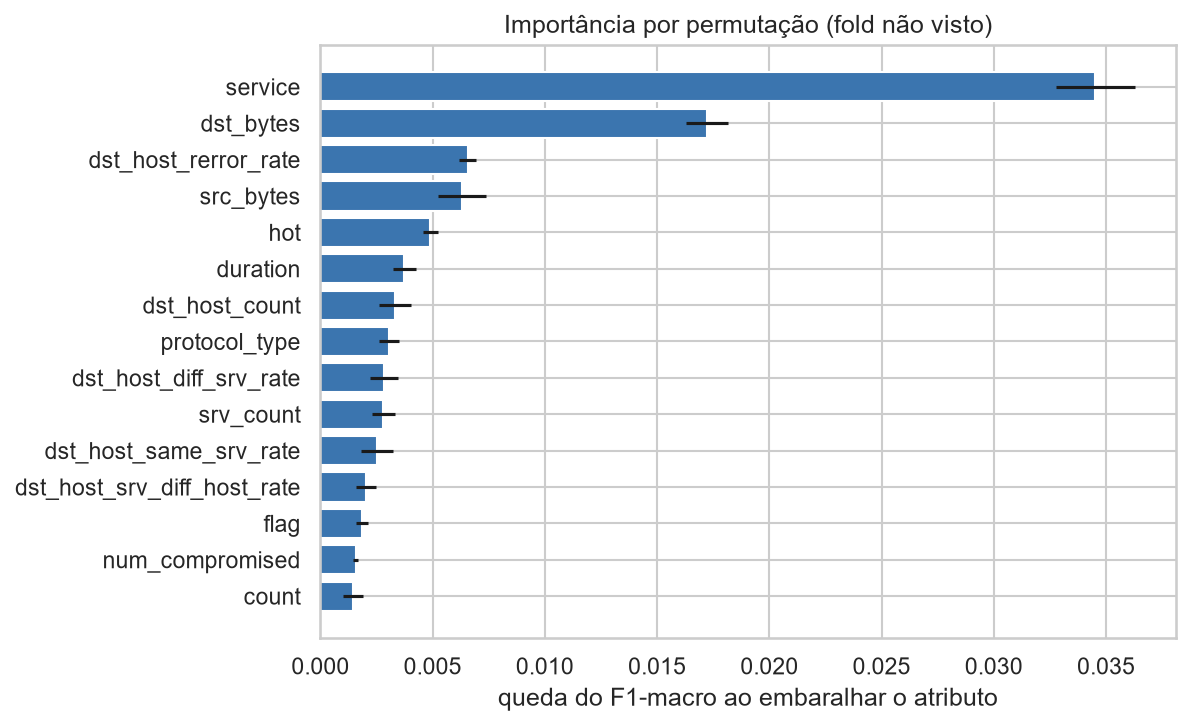
\includegraphics[width=\linewidth]{figuras/final_permutacao.png}
\end{minipage}\hfill
\begin{minipage}[c]{0.50\linewidth}
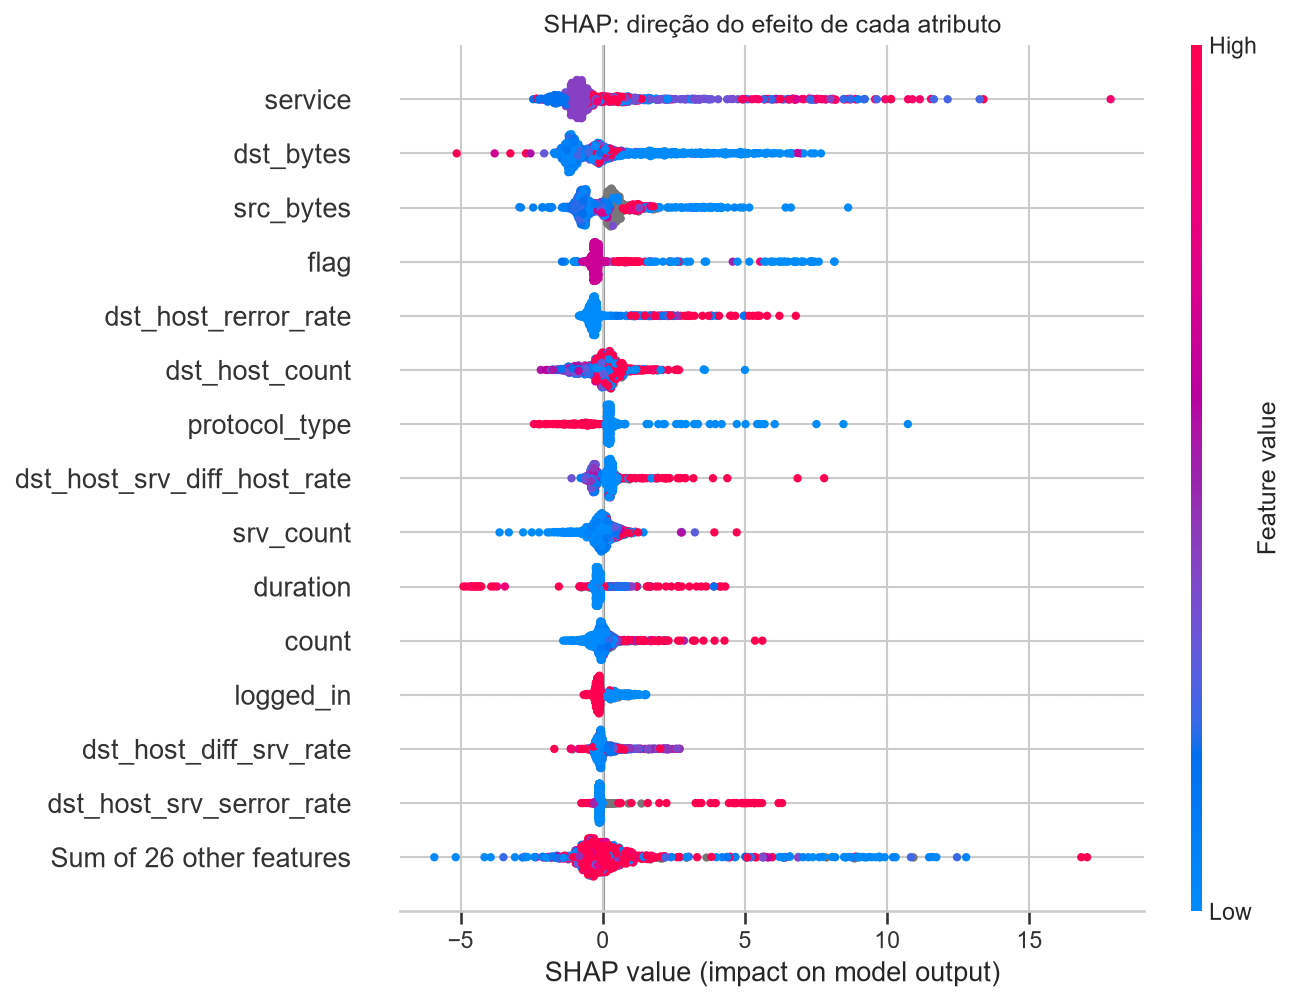
\includegraphics[width=\linewidth]{figuras/final_shap_beeswarm.png}
\end{minipage}
\caption{À esquerda, queda do F1-macro ao embaralhar cada atributo, num fold que o modelo não viu. À direita, SHAP: cada ponto é uma conexão; à direita do zero, o atributo empurrou para ataque; a cor é o valor do atributo.}
\label{fig:xai}
\end{figure}

\begin{itemize}
\item \textbf{Importância por permutação.} Embaralhar \texttt{service} derruba o F1-macro em 0,035, o maior efeito: muitos ataques miram serviços característicos (\texttt{private}, \texttt{ecr\_i}, \texttt{telnet}). Seguem os volumes de bytes e as taxas de erro por host.
\item \textbf{SHAP.} Concorda com a permutação no topo (\texttt{service}, \texttt{dst\_bytes}, \texttt{src\_bytes}) e mostra a direção dos efeitos: poucos bytes de resposta e taxas de erro de conexão altas empurram para ataque, como em varreduras e inundações de SYN; usuário autenticado (\texttt{logged\_in} = 1) empurra para normal. Usamos o explicador por permutação, porque verificamos que o \texttt{TreeExplainer} não reproduz as categorias nativas do HGB. Nos exemplos individuais, uma inundação de SYN (\texttt{flag} S0, 276 conexões em 2 segundos) recebe probabilidade 1,000, enquanto uma sessão \texttt{telnet} de ataque, sem nenhum sinal no tráfego, recebe 0,003: esse tipo de ataque é difícil de detectar só com estatísticas de tráfego.
\item \textbf{Árvore substituta.} Uma árvore de 4 níveis reproduz \textbf{98,4\%} das decisões do modelo. Suas regras são assinaturas conhecidas: quase todas as conexões ao serviço com erro de SYN indicam inundação de SYN; poucas conexões ao mesmo serviço, com muitos serviços diferentes ou rejeições, indicam varredura de portas; rajadas de ICMP indicam ataques como \emph{smurf}.
\end{itemize}

% =====================================================================
\section{Conclusão}

Construímos um detector de intrusão que usa apenas o tráfego de rede, escolhido e avaliado sem nenhum contato com o teste. As escolhas que mais contribuíram foram remover cópias e conflitos no ajuste (+0,004 de F1-macro), ajustar o limiar de decisão (+0,002 a +0,003) e usar um boosting que trata ausentes e categorias nativamente. Esperamos F1-macro de cerca de 0,88 no teste, se ele seguir o perfil do treino; o valor reflete o teto de 0,905 imposto pelos rótulos contraditórios, e não uma limitação do modelo. Abrimos mão de cerca de 0,015 no ranking ao excluir as colunas de vazamento, em troca de um modelo metodologicamente correto e que funcionaria na prática.

\section*{Declaração de uso de Inteligência Artificial}

Declaramos que a ferramenta de Inteligência Artificial Claude foi utilizada como apoio à revisão crítica das análises e dos procedimentos desenvolvidos pela equipe, bem como à formatação e ao aprimoramento da redação deste relatório, com o objetivo de verificar a consistência do trabalho realizado e melhorar a clareza, a organização e a apresentação textual das informações.

\end{document}
